\scanpage{151}
% archive foliation: 150
\deleted{il faut \unsure{en effet}} les $C_i$ sont non singulières
[car $\unsure{\mathrm{Pic}_{C_i/k}^0}$ est un quotient de $\mathrm{Pic}_{C/k}^0$] et \deleted{\unsure{que}}
\deleted{\unsure{les} $\mu'_\alpha$ \unsure{est le nbr des} $C_i$ qui passent par \unsure{$P_\alpha$},}
pour $i\ne j$, alors $C_i$ et $C_j$ se coupent en un pt au plus
[car $\mathrm{Pic}(C_i\cup C_j)$ est un quotient de $\mathrm{Pic}(C)$].
\deleted{Soit $\nu_\alpha$ le nbr des $C_i$ passant par $P_\alpha$, on a
\[
\begin{aligned}
\dim G_{\mathrm{mult}}&=\sum(\nu_\alpha-1)-c_0+1\\
&=\sum_i(\text{nbr des pts }P_\alpha\text{ sur }C_i-1)-
\end{aligned}
\]
}
Alors finalement, on trouve de cette façon que l'on ne peut avoir de cycles
\figure{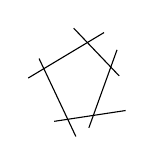
\begin{tikzpicture}[scale=.55]
\draw (-.35,.55)--(1.4,1.6); \draw (.7,1.7)--(1.75,.6);
\draw (1.7,1.2)--(1.05,-.6); \draw (1.9,-.2)--(.25,-.45);
\draw (-.1,1)--(.75,-.8);
\end{tikzpicture}}
dans le schém. combinatoire de $C$. \deleted{\unsure{(un arbre)},}
\unsure{Réciproqt}, si $C$ n'a que des pts \deleted{doubles}\inserted{multiples}
``multiplicatifs'', et si les $C_i$ sont non singuliers, on voit par récurrence sur le nb des $C_i$ que
\deleted{$C$} $\mathrm{Pic}_{C/k}^0$ \unsure{est} une V.A.

On aura en tous cas
\[
\begin{aligned}
g=\dim\mathrm{Pic}_{C/k}&=\sum g_i+(\sum_\alpha\mu_\alpha-c_0+1)\\
&=\sum g_i+\deleted{\unsure{h_1}}\rho+\sigma
\end{aligned}
\]
\margin{$g_i=\text{genre de }\widetilde C_i$}
$\rho=$ nb des cycles combinatoires, $+$ somme des \unsure{nbrs} des multiplicités multiplicatives des $C_i$
[\unsure{nulles donc} $=0$ si les $C_i$ non sing]

$\sigma=$ somme des multiplicités additives des $P_\alpha$.

